\chapter{Implementation and evaluation}
\label{chap:implementation}

\minitoc

To analyze the performance of a locking mechanism, it is essential to implement and evaluate it with a benchmark which simulates a real-world workload. In this chapter, we present an implementation of CALock and assess its performance using the STMBench7 benchmark \cite{guerraoui2006stmbench7}. STMBench7 is based on a CAD/CAM application and models a set of design objects into a hierarchy. 
We first provide an overview of the STMBench7 data model and then describe the implementation of CALock, focussing on the labelling mechanism, lock pool and conflict detection protocol. We compare the performance of CALock with coarse-grain locks, medium-grain locks, Intention Locks, DomLock, Multi-Interval DomLock, and Flexigran.

\section{Hierarchy schema for evaluation}

STMBench is a well-known benchmark based on the classical OO7 object-oriented benchmark suite \cite{CareyDN93}. It is widely used to evaluate the performance of hierarchical algorithms and data structures \cite{prokopec_renaissance_2019,vale_pot_2016, felber_hardware_2016, carvalho_optimizing_2016, kim_scheduling_2015,filipe_nested_2015,rito_props_2014,kalikar2016domlock,anjuMID, FlexiGran2024, KalikarN18, GaneshKN18, liu_unleashing_2014} 

\begin{figure}[h]
    \centering
    \captionsetup{justification=centering}
    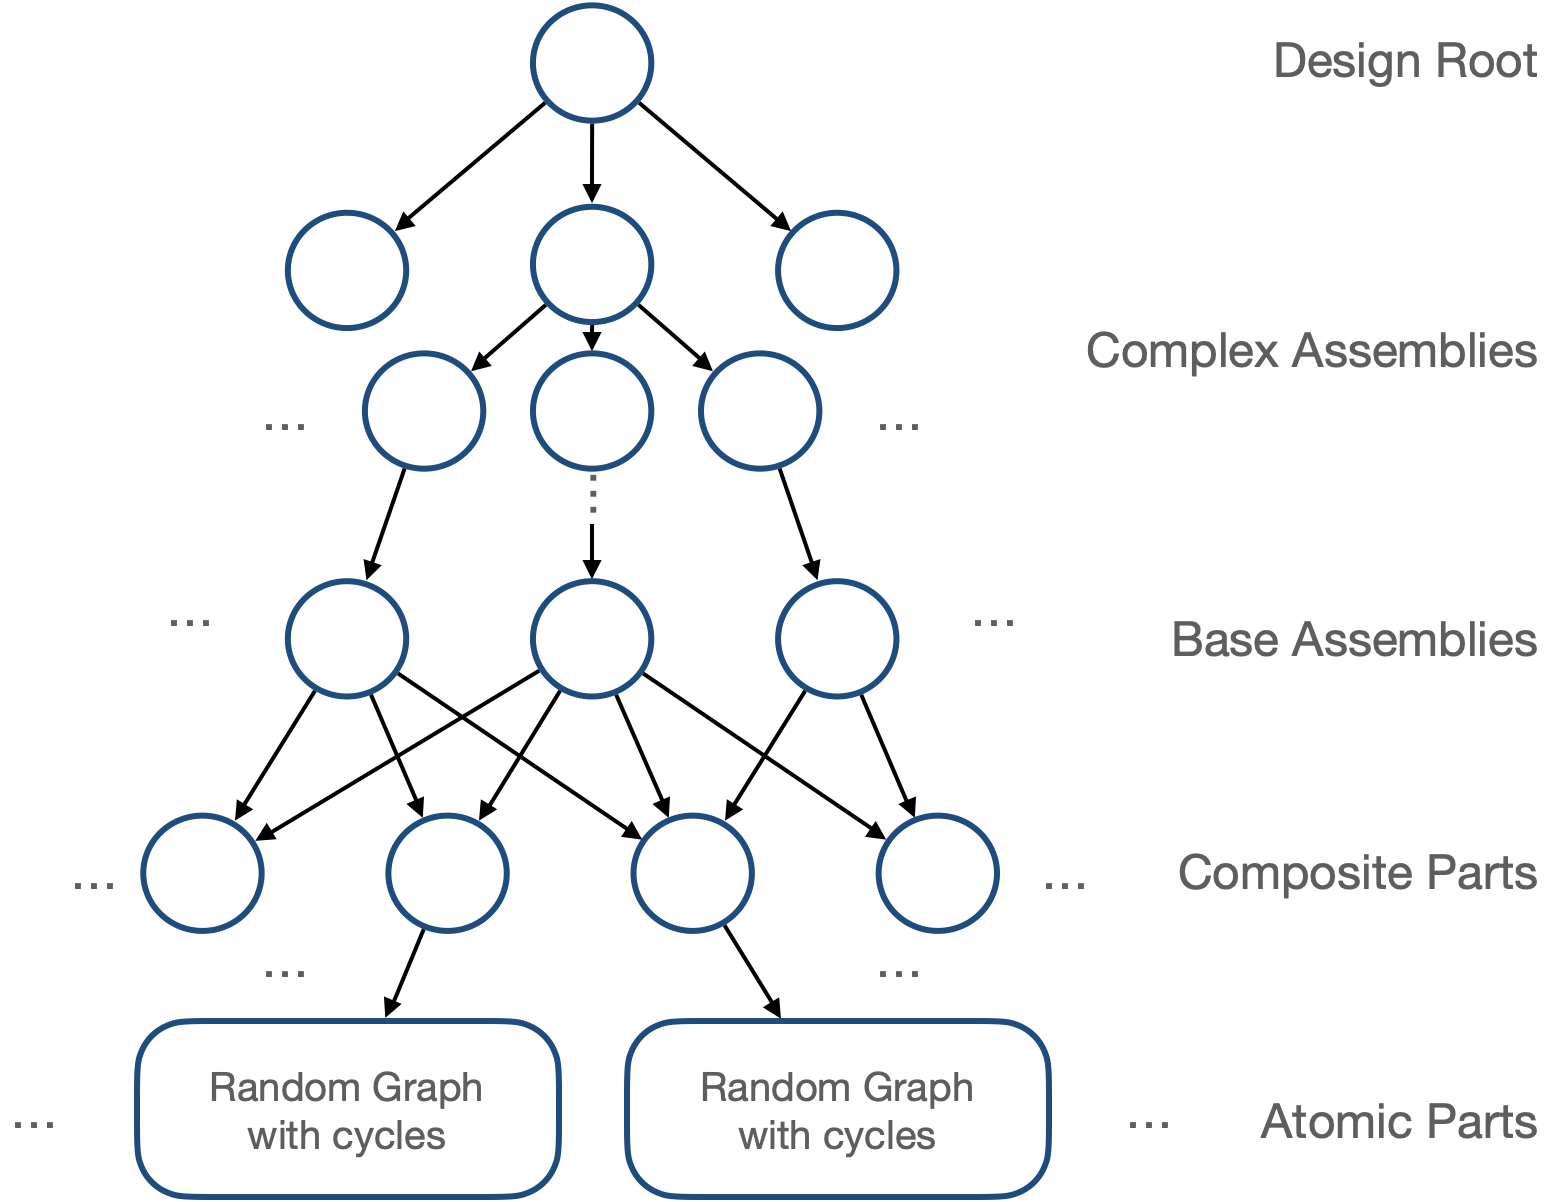
\includegraphics[width=.8\columnwidth]{figures/STMBenchModuleWithoutLocks.png}
    \caption{Structure of a module in STMBench with medium lock boundaries}
    \label{stmbenchModuleUnlocked}
\end{figure}

The hierarchy in STMBench7, as represented in \cref{stmbenchModuleUnlocked}, consists of a \emph{module} at the root level. This module consists of several levels of \emph{complex assemblies}. 
Each of the deepest complex assemblies consists of a set of \emph{base assemblies}. 
A \emph{composite part} can be contained in several base assemblies. 
Each composite part contains a set of \emph{atomic parts}. 
These atomic parts form a near-complete graph. 
The root of this graph is connected to a single composite part via a designated vertex called the \emph{root part}.
	



\section{Implementation of CALock}
The implementation of CALock written in C\texttt{++}, chosen for its ability to deliver high performance and fine-grained control over data structures. 
Several optimizations have been integrated to ensure the protocol operates efficiently. These include techniques to reduce the size of the labels, which conserve memory. Additionally, the implementation minimizes the number of index accesses required to locate the Lowest Guarding Common Ancestor (LGCA), a pivotal step in the locking protocol. These optimizations are designed to balance computational efficiency and scalability, making CALock suitable for hierarchical data structures with varying levels of structural complexity.

\subsection{CALock labelling}
\label{sec:calock-labelling}
The CALock labelling is implemented as the \texttt{CALockLabelling} class, which provides a method \texttt{run()} to label the graph. Unlike the protocol description in \cref{chap:CALock}, which uses characters as vertex IDs, our implementation uses integers. This allows for compact storage representation and faster membership tests. The hierarchy in STMBench consists of 4 different types of vertices. The implementation distinguishes each by assigning them an integer suffix based on their type. CALock IDs for vertices are constructed by appending this suffix to the STMBench vertex ID. The suffixes are as follows:

\begin{itemize}
    \item Complex Assembly: \texttt{<Identifier>::1}
    \item Base Assembly: \texttt{<Identifier>::2}
    \item Composite Part: \texttt{<Identifier>::3}
    \item Atomic Part: \texttt{<Identifier>::4}
\end{itemize}

Using this representation, a vertex with STMBench identifier 52 of type \texttt{Atomic Part} has a CALock ID 524.

\subsubsection{Vertex labels}

The label on each vertex is an ordered set containing the CALock IDs of the guarding ancestors of that vertex. In the implementation, to facilitate a fast membership test to detect conflicts as well as finding the LGCA, each vertex contains a \texttt{std::Set} of guarding ancestors and a \texttt{std::Vector} containing an order of these guarding ancestors.  \cref{lst:vertexClass} shows the \texttt{Vertex} class with the CALock label fields.

A \texttt{vector} in C\texttt{++} provides constant time insertion but is linear for a membership test. A search is performed to check if an element exists in a vector via the \texttt{std::find} function from the C\texttt{++} standard template library.

Since membership tests are frequently used in CALock when locking and conflict detection, the implementation uses an auxiliary \texttt{set} for membership tests. It bypasses the vector's linear search complexity. Together, a vector and a set provide constant-order time complexity for membership tests and label updates. The set and the vector are synchronized outside the critical path to contain the same CALock IDs.

\begin{lstlisting}[caption={Vertex class with CALock label fields}, label={lst:vertexClass}]
class Vertex {
    ...
    int id;
    bool hasLabel;
    vector<int> pathLabel{};
    set<int> guardingAncestors{};
    bool isDeleted;
    ...
};

\end{lstlisting}

% Using this class, the LGCA is computed by taking the last element of the path label. 

To find the LGA(lowest guarding ancestor) of a single vertex, the last element of the \lstinline{pathLabel} vector is returned (\cref{lst:lst:findLGA}). When finding the LGCA(lowest guarding common ancestor) of a set of vertices, the intersection of the path labels of the vertices is computed. The last element of the resulting vector is the LGCA. This is shown in \cref{lst:findLGCA}.

\begin{lstlisting}[caption={Finding LGA using path label}, label={lst:findLGA}]
int getLGA() const {
    if (pathLabel.size() == 1) {
        return *(--pathLabel.rbegin());
    } else {
        return *pathLabel.rbegin();
    }
}
\end{lstlisting}


\begin{lstlisting}[caption={Finging the LGCA of a set of atomic parts}, label={lst:findLGCA}]

int getLGCA(const vector<AtomicPart *> &aparts) const {
    list<int> guardingCommonAncestors{};
    auto it = aparts[0]->pathLabel.rbegin();
    auto end = aparts[0]->pathLabel.rend();
    for (auto i: aparts[0]->pathLabel) {
        for (auto a: aparts) {
            if (a->guardingAncestors.contains(i)) {
                guardingCommonAncestors.push_back(i);
            }
        }
    }
    return guardingCommonAncestors.rbegin();
}

\end{lstlisting}


\subsubsection{Labelling algorithm}

The labelling algorithm is a breadth-first traversal over the hierarchy. It is implemented by keeping separate queues for each vertex type: Complex Assembly, Base Assembly, Composite Part, and Atomic Part. The implementation is shown in \cref{lst:labelling-algo}.
Labelling starts from the root of the hierarchy. The root of the hierarchy is a Complex Assembly. First, we add a suffix to the root's ID to get the CALock ID. The CALock ID is then set as the root's label. The root is then added to the queue of Complex Assemblies to initiate the labelling process. 

All complex assemblies are labelled first using the function \texttt{traverse(cassmQ.front(), \&cassmQ, \&bassmQ)}. At the lowest level, complex assemblies contain base assemblies. While traversing, the algorithm labels the complex assembly and adds its children to the queue of complex assemblies (\texttt{cassmQ}) or base assemblies (\texttt{bassmQ}) based on their type. Once all complex assemblies are labelled, the algorithm proceeds to label base assemblies using function \texttt{traverse(bassmQ.front(), \&cpartQ)}. This process continues until all vertices are labelled.


\begin{lstlisting}[caption={BFS traversal for CALock labelling}, label={lst:labelling-algo}]
void CALockLabelling::run(int tid) const{
    queue<ComplexAssembly *> cassmQ;
    queue<BaseAssembly *> bassmQ;
    queue<CompositePart *> cpartQ;
    queue<AtomicPart *> apartQ;

    ComplexAssembly *root = dataHolder->getDesignRoot();
    vector<int> rootLabel = root->pathLabel;
    //Append Complex Assembly suffix (1) to the root ID to get CALock ID.
    rootLabel.push_back((root->getId() * 10) + 1);
    root->setPathLabel(rootLabel);
    cassmQ.push(root);
    // Label all complex assemblies.
    while (!cassmQ.empty()) {
        // Traverse a complex assembly and compute its label. Add its children to cassmQ or bassmQ
        traverse(cassmQ.front(), &cassmQ, &bassmQ);
        cassmQ.pop();
    }
    // Label all base assemblies.
    while (!bassmQ.empty()) {
        // Traverse a base assembly and compute its label. Add its children to cpartQ.
        traverse(bassmQ.front(), &cpartQ);
        bassmQ.pop();
    }
    // Label all composite parts.
    while (!cpartQ.empty()) {
        // Traverse a composite part and compute its label. Add its children to apartQ.
        traverse(cpartQ.front(), &apartQ);
        cpartQ.pop();
    }
}
\end{lstlisting}

The \texttt{traverse()} method is overloaded for each vertex type. After computing the label of a vertex, the method adds the children of the vertex into their appropriate queues based on their type. \cref{lst:traverseCA} shows the implementation of the \texttt{traverse()} method for a vertex of Complex Assembly type. The method traverses the children of a complex assembly and labels them. Each assembly gets a CALock ID by appending its type suffix to its STMBench ID. For instance, a base assembly is assigned an ID with suffix 2 (\texttt{int labelIdentifier = (assm->getId() * 10) + 2}).

\begin{lstlisting}[caption={Labelling a complex assembly},label={lst:traverseCA}]
void traverse(  ComplexAssembly *cassm, 
                queue<ComplexAssembly *> *cassmQ, 
                queue<BaseAssembly *> *bassmQ) const {

    list<int> currLabel = cassm->pathLabel;
    // Get the children of the complex assembly.
    Set<Assembly *> *subAssm = cassm->getSubAssemblies();
    SetIterator<Assembly *> iter = subAssm->getIter();
    bool childrenAreBase = cassm->areChildrenBaseAssemblies();

    while (iter.has_next()) {
        Assembly *assm = iter.next();
        if (!childrenAreBase) {
            // If children are Complex Assemblies, add them to the Complex Assembly queue.
            int labelIdentifier = (assm->getId() * 10) + 1;
            currLabel.push_back(labelIdentifier);
            // Set the label of the vertex.
            assm->setPathLabel(currLabel);
            cassmQ->push((ComplexAssembly *) assm);
        } else {
            // If children are Base Assemblies, add them to the Base Assembly queue.
            int labelIdentifier = (assm->getId() * 10) + 2;
            currLabel.push_back(labelIdentifier);
            // Set the label of the vertex.
            assm->setPathLabel(currLabel);
            bassmQ->push((BaseAssembly *) assm);
        }
        currLabel.pop_back();
    }
}
\end{lstlisting}



The Atomic Part graph in STMBench is dense and can contain many cycles. Due to this, atomic Parts are handled differently since an atomic part vertex can be visited multiple times. An atomic part graph is connected to the hierarchy under a composite part via a vertex called the \texttt{rootPart}. The \texttt{rootPart} is designated as the root of the atomic part graph. Once this root is labelled, the algorithm traverses the graph of atomic parts post-order. The implementation of the \texttt{traverse} method for an Atomic Part is shown in \cref{lst:traverseAP}. Labelling atomic parts terminates once their labels reach a fixpoint (lines 2-7). 

An atomic part stores a set of incoming and outgoing edges. The parents of an atomic part are located using the incoming edges (\texttt{apart->getFromConnections()}). The label of an atomic part is computed by successively removing guarding ancestors that are not present in the guarding ancestors of its parents. Once all the parents are tested, the atomic part is labelled with the guarding ancestors of its parents along with its own CALock ID. If the label of an atomic part changes, the algorithm recursively labels all children of the atomic part. 


\begin{lstlisting}[caption={Labelling an atomic part},label={lst:traverseAP}]
void traverse(AtomicPart *apart, Set<AtomicPart *> &visitedPartSet, list<int> currLabel) {
    if (visitedPartSet.contains(apart)) {
        return;
    } else {
        visitedPartSet.add(apart);
        Set<Connection *> *fromConns = apart->getFromConnections();
        SetIterator<Connection *> fiter = fromConns->getIter();
        // Find ancestors that are in the atomic part's label but are not guarding ancestors of its parents.
        set<int> removals;
        for (int a: currLabel) {
            bool allContain = true;
            while (fiter.has_next()) {
                if (!fiter.next()->getSource()->guardingAncestors.contains(a)) {
                    allContain = false;
                    break;
                }
            }
            if (!allContain) {
                removals.insert(a);
            }
            fiter = fromConns->getIter();
        }
        // Remove all ancestors which are not in the guarding ancestors of the parents.
        currLabel.remove_if([removals](int l) { return removals.contains(l); });

        if (currLabel != apart->pathLabel) {
            // If the label has changed, set the new label and label the children.
            apart->setPathLabel(currLabel);
            Set<Connection *> *toConns = apart->getToConnections();
            SetIterator<Connection *> iter = toConns->getIter();
            while (iter.has_next()) {
                Connection *conn = iter.next();
                currLabel.push_back((conn->getDestination()->getId() * 10) + 4);
                traverse(conn->getDestination(), visitedPartSet, currLabel);
                currLabel.pop_back();
            }
        }
        visitedPartSet.remove(apart);
    }
}
\end{lstlisting}




\subsection{Lock requests and the lock pool}

Once a thread wishes to lock a set of targets, it creates a lock request. The lock request is implemented as a \texttt{lockObject} inserted into the lock pool. This \texttt{lockObject} contains the following fields:

\begin{itemize}
    \item \texttt{int Id}: Guard ID.
    \item \texttt{set<int> *guardingAncestors}: Set of guarding ancestors.
    \item \texttt{int mode}: Mode of the lock (Read/Write).
    \item \texttt{long Oseq}: Sequence number to decide the arrival order of the lock requests.
    \item \texttt{atomic\_flag accessController}: Flag which conflicting threads use to wait on this thread.
\end{itemize}

The \texttt{lockObject} class is shown in \cref{lst:lock-object}. The \texttt{atomic\_flag} type is an atomic boolean, provided by C\texttt{++} and is guaranteed to be lock-free. Operations on this type are guaranteed to occur in the same order as they are issued and are not reordered by compiler optimizations. This prevents nondeterministic thread blocks due to release/acquire reordering on some CPU architectures. Multiple atomic flags within the same program are totally ordered, preventing blocked threads from being notified before the lock is released.

\begin{lstlisting}[caption={\texttt{lockObject} class}, label={lst:lock-object}]
class lockObject {
public:
    set<int> *guardingAncestors;
    int Id;
    int mode;
    long Oseq;
    atomic_flag accessController = ATOMIC_FLAG_INIT;

    lockObject(int pId, set<int> *ancestors, int m) {
        Id = pId;
        guardingAncestors = ancestors;
        mode = m;
        Oseq = -1;
        accessController.test_and_set();
    }
};
\end{lstlisting}

The lock pool is an array that contains \texttt{lockObjects}. The size is fixed and bounded to the number of concurrent hardware threads the system provides. \cref{lst:lock-pool} shows the class definition of the CALock lock pool.

\begin{lstlisting}[caption={\texttt{lockPool} class}, label={lst:lock-pool}]
class CAPool {
public:
    mutex lockPoolLock;
    lockObject *locks[SIZE];
    shared_mutex threadMutexes[SIZE];
    condition_variable_any threadConditions[SIZE];
    long int Gseq;

    CAPool() {
        Gseq = 0;
        for (int i = 0; i < SIZE; i++) {
            locks[i] = nullptr;
        }
    }
    bool acquireLock(lockObject *reqObj, int threadID) {
        //Check for conflicts and wait for resolution
    }
    void releaseLock(lockObject *l, int threadId) {
        //Release the lock
    }
};
\end{lstlisting}


When acquiring a lock, a thread inserts a \texttt{lockObject} corresponding to its lock request into the pool and waits for the lock to be granted. The \texttt{acquireLock} method checks for conflicts and waits for resolution. The method is shown in  \cref{lst:acquire-lock}.

\begin{lstlisting}[caption={Acquiring a lock on \texttt{reqObj}}, label={lst:acquire-lock}]
bool acquireLock(lockObject *reqObj, int threadID) {
    lockPoolLock.lock();
    reqObj->Oseq = ++Gseq;
    locks[threadID] = reqObj;
    lockPoolLock.unlock();
    for (int i = 0; i < SIZE; i++) {
        // A thread won't run into conflict with itself.
        if (locks[i] != nullptr) {
            auto l = locks[i];
            if (l != nullptr &&
                // Mode Conflict.
                (reqObj->mode == 1 || l->mode == 1) &&
                // Grain Overlap.
                (reqObj->Id == l->Id ||
                reqObj->guardingAncestors->contains(l->Id) ||
                l->guardingAncestors->contains(reqObj->Id)) &&
                // Arrival Order.
                (reqObj->Oseq > l->Oseq)) {
                // Wait for resolution and notification.
                l->accessController.wait(true);
            }
        }
    }
    return true;
}
\end{lstlisting}

A lock request is first assigned its sequence number (\texttt{Oseq}) and then inserted into the lock pool. This assignment and insertion into the pool is done under a mutex lock on the pool to prevent a race condition between the assignment of a sequence number and insertion into the pool ( \cref{lst:acquire-lock} - lines 2-5).

Once a lock request is inserted into the pool, the method checks for conflicts with other lock requests by iterating over the pool from left to right. This check can be performed in parallel for all lock requests in the pool. The lock is granted if no conflict is detected, and the thread can proceed.

If a conflict is detected, the thread waits until the conflicting request releases its lock. This is done by waiting on the \texttt{accessController} of a conflicting lock request flag to become \texttt{false} ( \cref{lst:acquire-lock} - line 21). Even when present in the lock pool, a request with activity indicator \texttt{false} is considered to have released its lock.


\begin{lstlisting}[caption={Releasing a lock}, label={lst:release-lock}]
    void releaseLock(lockObject *l, int threadId) {
        locks[threadId] = nullptr;
        l->accessController.clear();
        l->accessController.notify_all();
    }
\end{lstlisting}

When a thread releases a lock, it removes the lock request from the pool, changes its \texttt{accessController} flag to \texttt{false}, and notifies all waiting threads. The \texttt{releaseLock} method is shown in  \cref{lst:release-lock}. Once waiting threads are notified, they resume execution and check for further conflicts in the lock pool.


After checking for conflicts with all lock requests in the pool and waiting on conflicting requests, a thread reaches the end of the lock pool ( \cref{lst:acquire-lock} - line 6). At this point, the lock is always granted, as there are two possible scenarios:

\begin{enumerate}
    \item[\textbf{a}.] The lock request does not conflict with any other lock request in the pool ( \cref{lst:acquire-lock} - lines 12, 13).
    \item[\textbf{b}.] The lock request has priority over all conflicting lock requests in the pool because its sequence number is smaller than all conflicting lock requests ( \cref{lst:acquire-lock} - line 19). 
\end{enumerate}



\subsection{Overall execution of an operation in CALock}

The overall execution of an operation in CALock is shown in  \cref{lst:overall-execution}. The operation is executed in the \texttt{run()} method of the \texttt{operation} class. The listing shows a structural modification in which a composite part is added to a base assembly.

This operation first computes the set intersection of the labels of the base assembly and the composite part. This set intersection finds the LGCA of the base assembly and composite part.( \cref{lst:overall-execution} - lines 8-19).

A lock request is created with the LGCA and the guarding ancestors in write mode ( \cref{lst:overall-execution} - line 21). The lock is acquired using the \texttt{acquireLock()} method of the lock pool. The thread waits for resolution as long as the lock is not granted ( \cref{lst:overall-execution} - line 24). Once granted, the operation is performed ( \cref{lst:overall-execution} - line 26).

Since a structural modification has occurred, the hierarchy is relabelled. This is done by executing a relabelling operation and adding the composite part to the queue of parts for relabelling ( \cref{lst:overall-execution} - lines 28-30). 

After relabelling is complete, the lock is released via the \texttt{releaseLock()} method of the lock pool ( \cref{lst:overall-execution} - line 32).


\begin{lstlisting}[caption={Overall execution of an operation in CALock}, label={lst:overall-execution}]
int CAStructuralModification3::run(int tid) const {
    CompositePart *cpart = dataHolder->getCompositePart(cpartId);
    BaseAssembly *bassm = dataHolder->getBaseAssembly(bassmId);

    list<int> lockLabel = {};

    // Find the set intersection of the labels of bassm and cpart.
    for (int a: bassm->pathLabel) {
        if (cpart->guardingAncestors.contains(a)) {
            lockLabel.push_back(a);
        }
    }

    // find the LGCA of the bassm and cpart.
    pair<DesignObj *, bool> lo = lscaHelpers::getLockObject(lockLabel);
    //if cassm is disconnected, use bassm as the LGCA.
    if (!lo.second) {
        lo.first = bassm;
    }
    //create a lock request with the LGCA and the guarding ancestors in write mode. 
    auto *l = new lockObject(lo.first->getLabellingId(), &lo.first->guardingAncestors, 1);

    // Acquire the lock.
    if (caPool.acquireLock(l, tid)) {
        // Perform the operation.
        bassm->addComponent(cpart);
        // Relabel the hierarchy because a structural modification has occurred.
        auto *r = new CALockRelabeling(dataHolder, tid);
        r->cpartQ.push(cpart);
        r->run();
        // Release the lock.
        caPool.releaseLock(l, tid);
    }

}

\end{lstlisting}


% !TEX root = ../../main.tex



\section{Performance evaluation of CALock} \label{chap:evaluation}

% \minitoc

To evaluate the performance of CALock and experimentally compare it with the state of the art, we perform several macro and micro-benchmarks. Our evaluation uses the same benchmark as DomLock, MID and FlexiGran \cite{kalikar2016domlock,anjuMID,FlexiGran2024} i.e. STMBench7\cite{guerraoui2006stmbench7}. In this section, we first present the experimental setup and then the results of the experiments and discuss their implications. 

\subsection{Experimental setup and codebase}

We run our experiments on a machine with an AMD EPYC 7642 CPU, with 48 Cores, a base clock of 2.3 GHz and 512 GB of RAM \footnote{Experiments presented in this thesis were carried out using the Grid'5000 testbed, supported by a scientific interest group hosted by Inria and including CNRS, RENATER and several Universities as well as other organizations (see https://www.grid5000.fr).}. 
The benchmark is deployed on a Docker container under Ubuntu 20.04. 
GCC 12.1 and Cmake 3.22 are used to build the benchmark. The compilation is done at the C\texttt{++} 23 standard to enable atomic wait primitives. The optimization level is set to O3.

The implementation of STMBench7  and all the lock protocols is open source and available in a \href{https://anonymous.4open.science/r/CALockBench-B117/Readme.md}{\color{blue}\underline{repository}}. The implementation contains scripts to configure the parameters, execute the benchmark and create performance charts. Optional raw data collection facilitates an in-depth understanding of the benchmark results.


\subsection{Benchmark suite: STMBench7}
	
STMBench7 provides coarse-grain and medium-grain lock implementations. These are representatives of fixed granularity locking techniques.   
The coarse-grain lock is a read-write lock on the entire graph. 
\cref{stmbenchModule} shows the medium-grain lock grains for a module. 
Complex assemblies are divided into levels, each guarded by its own lock.
Deeper in the graph, the set of atomic parts under each composite part is guarded by its own lock.
A structural modification operation acquires a mutex on the entire graph. STMBench provides a set of operations that stress the locking mechanism being evaluated. 

\begin{figure}
    \centering
    \captionsetup{justification=centering}
    \includegraphics[width=.9\columnwidth]{figures/STMBenchModule.png}
    \caption{Structure of a module in STMBench with medium lock boundaries}
    \label{stmbenchModule}
\end{figure}


% From these operations, Q1 and Q2 are read-only operations, OP1 and OP2 are read-write operations, OP3 and OP4 are write-only operations and SM1 and SM2 are structural modifications.

\paragraph{Read-only operations}

\begin{enumerate}
\item[\textbf{Q1}] Reading an atomic part
\item[\textbf{Q2}] Reading a set of atomic parts
\item[\textbf{OP1}] Reading a set of complex assemblies
\item[\textbf{OP2}] Reading a set of base assemblies
\end{enumerate}

\paragraph{Write-only operations}
\begin{enumerate}
\item[\textbf{OP3}] Writing data to an atomic part
\item[\textbf{OP4}] Writing data to a set of atomic parts
\end{enumerate}

\paragraph{Structural modifications}
\begin{enumerate}
\item[\textbf{SM1}] Deleting a composite part
\item[\textbf{SM2}] Adding an edge between a base assembly and a composite part
\end{enumerate}



\subsection{Synopsis}
To evaluate CALock, we compare it with coarse-grain locks, medium-grain locks, Intention locks, DomLock, MID and FlexiGran. To this end, we formulate research questions that scrutinize different aspects of the lock mechanism and address the claims made throughout this thesis. The questions we address are the following:

\begin{description}
		\item[\S \ref{benchmark:PerOpLatency}] How quickly does CALock grant a lock compared to other approaches for different operation types (Q1-SM2)?
		
		\item[\S \ref{benchmark:labellingAndRelabelling}] What is the cost of labelling a hierarchy with CALock labels compared to integer intervals for DomLock, MID and FlexiGran?
		
		\item [\S \ref{benchmark:metadatasize}] How expensive is it to maintain a set of guarding ancestors for each vertex in the hierarchy for CALock compared to integer intervals for DomLock, MID and FlexiGran? 
	
		\item[\S \ref{benchmark:falseSubsumption}] Does CALock eliminate false subsumptions and reduce grain size compared to DomLock, MID and FlexiGran?
		%\item(\S \cref{benchmak:ThreadIdling}) How long does a thread spend waiting for a lock?
		% \item[\S \cref{benchmark:lockRequestSize}] How does the size of a lock request affect the cost of locking?
		% \item[\S \cref{benchmar:lockLocality}] How does lock locality affect performance?
		\item[\S \ref{benchmark:StaticOverallPerf}] What is the performance of CALock compared to other lock strategies for workloads with only data updates (Q1-OP4)?
	
		\item[\S \cref{benchmark:DynamicOverallPerf}] What is the performance of CALock compared to other lock strategies for workloads that also include structural modifications (Q1-SM2)?
	\end{description}
	
	
\subsection{Per operation response time} \label{benchmark:PerOpLatency}

\paragraph{Question:} \emph{How quickly does CALock grant a lock compared to other approaches for different operation types (Q1-SM2)?}

\cref{ttc} shows the time to completion for different operations in STMBench7. 
Coarse-grain and medium-grain locks are the fastest at granting lock requests. However, they do not scale well (see \cref{benchmark:StaticOverallPerf}, \cref{benchmark:DynamicOverallPerf}). 

Intention locks are slower than coarse-grain and medium-grain locks because they require a depth-first traversal to acquire intention locks on the paths that lead to a target vertex. The cost of acquiring intention locks is linear in the number of unique paths to a target vertex. This cost is multiplied for requests with multiple target vertices (Q2, OP4), which leads to a higher response time. 

\begin{figure}[h]
	\captionsetup{justification=centering}
	\centering
	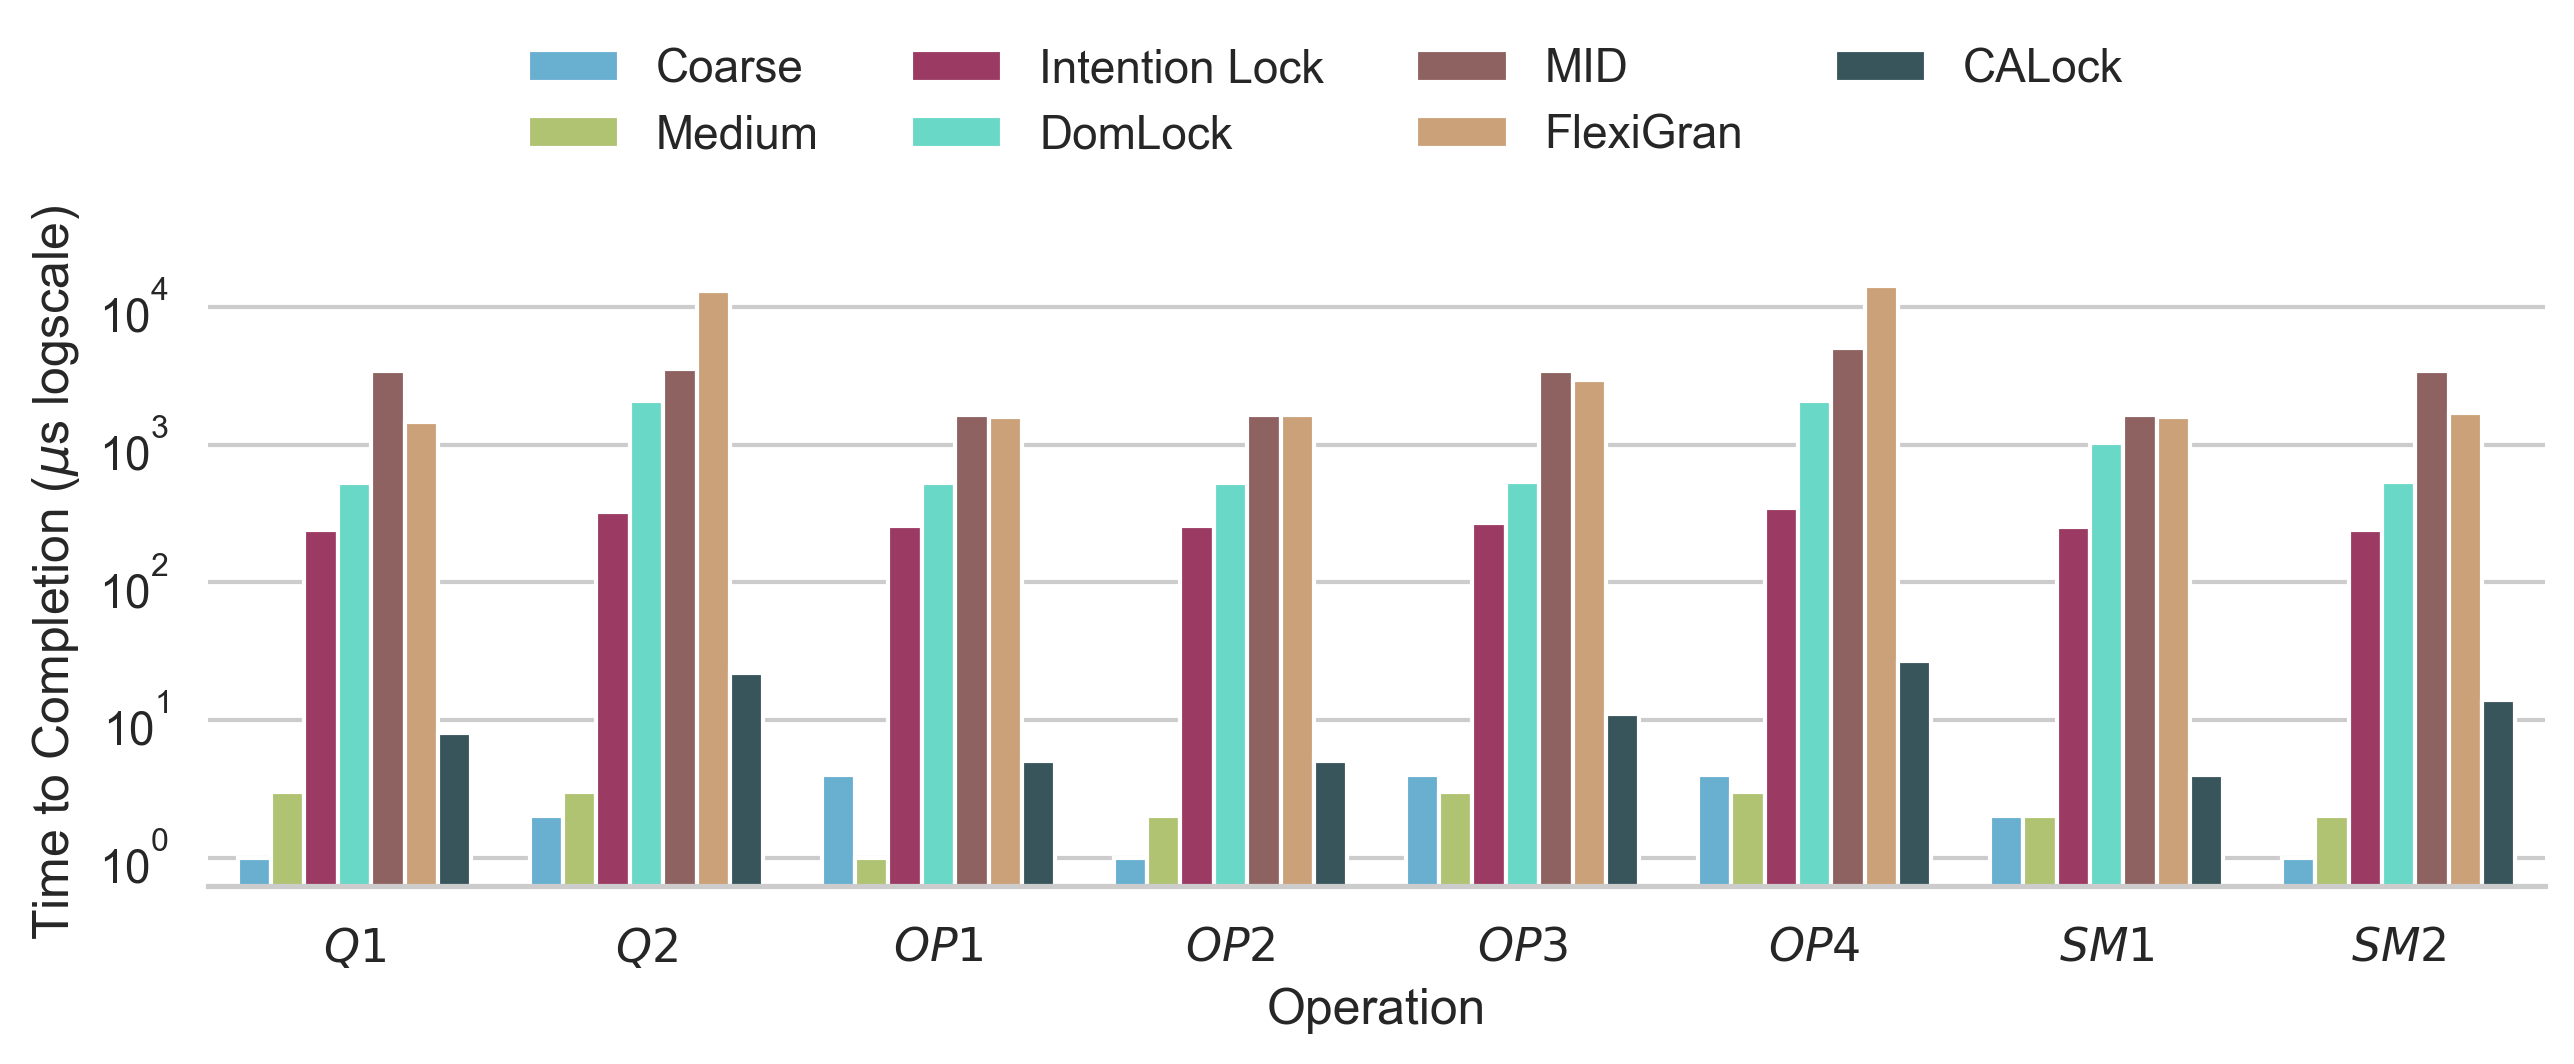
\includegraphics[width=\columnwidth]{figures/PerformanceCharts/TTC}
	\caption{Time to completion for different operations in STMBench (lower is better)}
	\label{ttc}
\end{figure}

In MGL techniques like DomLock, MID and FlexiGran, the time to completion is at least 300 times higher than coarse-grain, medium-grain and intention locks. Once a thread identifies the lock targets and finds their subsuming interval, a depth-first traversal is required to find the lock guard with the same interval. This traversal is especially expensive for vertices deeper in the hierarchy.


Between existing MGL techniques, DomLock is the fastest since conflict detection requires only testing overlap between a pair of intervals. MID is slower than DomLock because it involves testing overlap between a pair of intervals. FlexiGran is slower than MID because it requires testing overlap between intervals and level numbers. Conflict detection in FlexiGran MGL and FlexiGran fine-grained locks involves testing reachability between the guard of the MGL lock and the fine-grained lock. This is expensive and leads to a longer overall completion time.

CALock is at least 100 times faster to grant a lock than existing MGL techniques. This is because CALock eliminates needing a traversal to find the lock guard. Instead, a set intersection of the labels is used to find the LGCA, which serves as the lock guard. This is significantly faster than the depth-first traversal required by Intention locks, DomLock, MID and FlexiGran.

Read-only operations (Q1 and Q2) are the fastest since they can progress in parallel, even in the same grain. 
Write operations (OP3, OP4) are slower since they require exclusive access to the grain. Structural modifications often take the longest since they require exclusive access to the entire graph with DomLock, MID and FlexiGran. CALock parallelizes the relabelling of disjoint subgraphs and is at least 100 times faster. 



\subsection{Metadata management: preprocessing and relabelling} \label
{benchmark:labellingAndRelabelling}
 
\paragraph{Question:} \emph{What is the cost of labelling a hierarchy with CALock labels compared to integer intervals for DomLock, MID and FlexiGran?}

MGL techniques rely on metadata to identify lock grains. DomLock and MID use integer intervals for subsumption testing, and FlexiGran combines intervals with a level number. CALock, on the other hand, utilizes sets of vertex identifiers. Regardless of the metadata type, excessive housekeeping to maintain its accuracy can quickly negate any performance benefits. In this section, we examine the time required to compute the metadata initially (preprocessing) and the time needed to update it after a structural modification (relabelling). The benchmark is run on three different sizes of the STMBench7 graph. \cref{tab:graphSizes} lists the size of the STMBench7 hierarchies.

\begin{table}[h]
	\centering
	\captionsetup{justification=centering}
	\begin{tabular}{c|ll}
		\textbf{Graph Size} & \textbf{Vertices} & \textbf{Edges} \\ \hline
		Small  & 234,737 	& 4,393,682 	\\
		Medium & 2,334,257 	& 43,759,682	\\
		Large  & 23,329,457 & 437,419,682 	\\
	\end{tabular}
	\caption{Sizes of the STMBench7 hierarchies}
	\label{tab:graphSizes}
\end{table}


\subsubsection{Preprocessing}
We measure the preprocessing time, i.e., the time it takes to assign the labels to a graph for label-based MGL techniques like DomLock, MID, FlexiGran and CALock.
This simulates loading data into a database.
This time is measured for three different sizes of the STMBench7 graph. 
The results are shown in \cref{initialLabelling}. 
DomLock is the fastest since a single depth-first-traversal is sufficient to compute the intervals. MID is 8 times slower than DomLock because it needs to compute a pair of intervals for each vertex. One is computed by a depth-first traversal and another by a depth-first traversal on the mirror image of the graph. FlexiGran is faster than MID but slightly slower than DomLock because of the additional level information that needs to be computed per vertex. 

CALock takes the longest to preprocess a hierarchy since a recursive breadth-first traversal with a fix-point dependent on the number of paths to a vertex from the root defines the labels. CALock remains 10 times slower than MID and 20 times slower than DomLock for preprocessing. 

\begin{figure}
	\centering
	\captionsetup{justification=centering}
	\includegraphics[width=.7\columnwidth]{figures/PerformanceCharts/InitialLabelling}
	\caption{Time to compute initial labels (lower is better)}
	\label{initialLabelling}
\end{figure}


\subsubsection{Relabelling}
This benchmark studies the average time spent relabelling the graph per structural modification. Coarse grain, medium grain locks and intention locks do not have additional metadata and, hence, do not require relabelling. 
DomLock, MID and FlexiGran are significantly slow since they relabel the entire graph after a structural modification. This relabelling is performed under a global write lock and cannot be parallelized. \cref{relabellingTime} shows the time DomLock, MID, FlexiGran and CALock take to relabel the graph after a structural modification.

CALock relabels only the subgraphs directly affected by the structural modification under the same lock as the structural modification.
Thus, multiple grains can be locked, modified and relabelled in parallel. CALock is at least 100 times faster at relabelling than DomLock, MID and FlexiGran.

%\todo{Change figure 9 With the updated results after the run is complete on grid5000}
\begin{figure}[ht]
	\captionsetup{justification=centering}
	\centering
	% \begin{subfigure}[b]{.325\textwidth}
		% \includegraphics[width=\columnwidth]{PerformanceCharts/ReadWithModificationsRelabelling}
		% \caption{R:90\%,W:9.9\%,SM:0.1\%}
	% \end{subfigure}
	% \begin{subfigure}[b]{.32\textwidth}
	% 	\includegraphics[width=\columnwidth]{PerformanceCharts/BalancedWithModificationsRelabelling}
	% 	\caption{R:60\%,W:39.6\%,SM:0.4\%}
	% \end{subfigure}
	% \begin{subfigure}[b]{.32\textwidth}
		\includegraphics[width=.7\columnwidth]{figures/PerformanceCharts/ReadWithModificationsRelabelling}
	% 	\caption{R:10\%,W:89.1\%,SM:0.9\%}
	% \end{subfigure}
	\caption{Time spent relabelling the graph per structural modification (lower is better)}
	\label{relabellingTime}
\end{figure}

%\todo{Make another benchmark to graph the relabelling time for different types of vertices similar to the subsumption benchmark in \cref{nodesLockedPerNodeType}}

\subsection{Metadata size in memory} \label{benchmark:metadatasize}

\paragraph{Question:} \emph{How expensive is it to maintain a set of guarding ancestors for each vertex in the hierarchy for CALock compared to integer intervals for DomLock, MID and FlexiGran?}

Label-based MGL techniques utilize metadata to identify the lock grains.
DomLock utilizes compact integer ranges as labels. 
MID uses a pair of integer ranges to represent the intervals of the vertices.
FlexiGran uses the DomLock intervals and an integer to store the level of a vertex.
In contrast, CALock employs sets of vertex identifiers as labels, leading to a larger memory footprint.

\begin{figure}
	\centering
	\captionsetup{justification=centering}
	\includegraphics[width=.7\columnwidth]{figures/PerformanceCharts/LabelsMemorySize.png}
 	\caption{Size of the metadata used for labelling(lower is better)}
	\label{metadataSize}
\end{figure}

As shown in \cref{metadataSize}, CALock's metadata consumes approximately 1.5 times more memory than DomLock, MID and FlexiGran.
In DomLock, MID and FlexiGran, regardless of the topology of the graph, the label at each vertex consists of integers.
This has a low memory requirement. However, the exact topology of the hierarchy cannot be inferred from the labelling itself, leading to false subsumptions.
CALock labels, being sets, contain more information, allowing for smaller grain sizes and eliminating false subsumptions.



\subsection{Lock granularity and false subsumptions}\label{benchmark:falseSubsumption}

\paragraph{Question:} \emph{Does CALock eliminate false subsumptions and reduce grain size compared to DomLock, MID and FlexiGran?}

Locking a vertex in MGL implicitly also locks all other vertices present in the lock grain. This allows threads to use a single guard for multiple targets such that the guard is the root of the smallest sub-graph containing the targets. A smaller grain size allows more parallelism and reduces the probability of conflicts. 

We measure the number of targets implicitly locked for a guard vertex in the STMBench7 graph to compare the grain sizes for different locking protocols. 
\cref{nodesLockedPerNodeType} compares the average granularity per vertex type for locks acquired using DomLock, MID, FlexiGran and CALock.

\begin{figure}[h]
	\centering
	\captionsetup{justification=centering}
	\includegraphics[width=.7\columnwidth]{figures/PerformanceCharts/ContainmentRatio}
	\caption{Vertices locked per vertex type (lower is better)}
	\label{nodesLockedPerNodeType}
\end{figure}

Locking an atomic part has almost the same effect with all algorithms, with CALock marginally reducing grain sizes. 
When locking higher up in the graph, the effects vary. 
Locking a complex assembly is more expensive with DomLock, MID and FlexiGran because complex assemblies often share composite parts. Using a complex assembly as a lock guard causes all shared composite parts to be locked, leading to large grains. With DomLock, MID and FlexiGran, the grain size is 8 times bigger than CALock due to false subsumptions. 

When locking base assemblies with DomLock, MID and FlexiGran, multiple base assemblies are locked due to the one-to-many relationship between base assemblies and composite parts due to false subsumptions. CALock is significantly better at this level, with grain sizes 100 times smaller than DomLock, MID, and FlexiGran.

Composite parts exhibit a similar trend to base assemblies. CALock has a grain size 100 times smaller than DomLock, MID and FlexiGran. When a composite part is a lock target, the guard is often a base assembly or complex assembly because a composite part is usually contained in multiple base assemblies. Combined with false subsumptions, this leads to large grain sizes for DomLock, MID and FlexiGran.

The granularity of the lock and its effect on subsumption is highly dependent on the topology of the graph. 
False subsumptions aggravate the problem of large grains and lead to more grain overlaps between threads. 
The grain sizes of CALock are always smaller than other locking techniques, as is evident in \cref{nodesLockedPerNodeType}.


\subsection{Overall locking performance}

% Sections \cref{benchmark:PerOpLatency}, \cref{benchmark:labellingAndRelabelling}, \cref{benchmark:metadatasize} and \cref{benchmark:falseSubsumption} study individual parameters in isolation. Here, we study them together and evaluate their effects on overall performance. 
In the previous sections, we analyzed specific parameters individually: per-operation latency (\cref{benchmark:PerOpLatency}), labelling and relabelling time (\cref{benchmark:labellingAndRelabelling}), metadata size (\cref{benchmark:metadatasize}), and false subsumption ratio (\cref{benchmark:falseSubsumption}). In this section, we combine these parameters to study their collective impact on overall performance, providing a more comprehensive evaluation of runtime evaluation. 

% For FlexiGran, the percentage of fine-grain locks is set to 50\% as recommended by the authors in their paper \cite{FlexiGran2024}. 
In this set of benchmarks, we study data updates and structural modifications. 
Figures \cref{staticPerf} and \cref{dynamicPerf} show the throughput of workloads with data access only and workloads with structural modifications, respectively. 
The charts in these figures are plotted with the number of concurrent threads on the x-axis and the throughput (op/s) or response time ($\mu s$) on the y-axis. 
Response time is measured from when the thread issues a lock request until the lock is granted.


\subsubsection{Data access} \label{benchmark:StaticOverallPerf}
\paragraph{Question:} \emph{What is the performance of CALock compared to other lock strategies for workloads with only data updates (Q1-OP4)?}

% \begin{figure*}
% 	\centering
% 	\includegraphics[width=.9\textwidth]{figures/PerformanceCharts/Legend}
% \end{figure*}

\begin{figure*}
	\centering
	\captionsetup{justification=centering}
	\begin{subfigure}[b]{\textwidth}
		\centering
		\includegraphics[width=\textwidth]{figures/PerformanceCharts/Legend}
	\end{subfigure}
	\begin{subfigure}{.33\textwidth}
		\includegraphics[width=\textwidth]{figures/PerformanceCharts/ReadWithoutModificationsThroughput}
		\caption{R:90\%,W:10\%}
		\label{rwm}
	\end{subfigure}
	\begin{subfigure}{.32\textwidth}
		\includegraphics[width=\textwidth]{figures/PerformanceCharts/BalancedWithoutModificationsThroughput}
		\caption{R:60\%,W:40\%}
		\label{bwm}
	\end{subfigure}
	\begin{subfigure}{.32\textwidth}
		\includegraphics[width=\textwidth]{figures/PerformanceCharts/WriteWithoutModificationsThroughput}
		\caption{R:10\%,W:90\%}
		\label{wwm}
	\end{subfigure}
	\begin{subfigure}[b]{\textwidth}
		\caption*{\cref{rwm}, \cref{bwm}, \cref{wwm}: Throughput (higher is better)}
	\end{subfigure}


	\begin{subfigure}[b]{.33\textwidth}
		\includegraphics[width=\textwidth]{figures/PerformanceCharts/ReadWithoutModificationsIdleness}
		\caption{R:90\%,W:10\%}
		\label{irwm}
	\end{subfigure}
	\begin{subfigure}[b]{.32\textwidth}
		\includegraphics[width=\textwidth]{figures/PerformanceCharts/BalancedWithoutModificationsIdleness}
		\caption{R:60\%,W:40\%}
		\label{ibwm}
	\end{subfigure}
	\begin{subfigure}[b]{.32\textwidth}
		\includegraphics[width=\textwidth]{figures/PerformanceCharts/WriteWithoutModificationsIdleness}
		\caption{R:10\%,W:90\%}
		\label{iwwm}
	\end{subfigure}
	\begin{subfigure}[b]{\textwidth}
		\caption*{\cref{irwm}, \cref{ibwm}, \cref{iwwm}: Average time to grant lock request (lower is better)}
	\end{subfigure}



	\caption{Performance with different workload types on static graphs (R: reads, W: writes).}
	\label{staticPerf}
	\end{figure*}
Throughput figures \cref{rwm}, \cref{bwm} and \cref{wwm} show that coarse-grain and medium-grain locks have better throughput for up to 4 concurrent threads due to the additional computation of the lock grain required for DomLock, MID, FlexiGran and CALock. Beyond 4 threads, MGL techniques give better throughput. However, the performance of DomLock and MID stagnates at 8 threads.

The graph in STMBench is irregular and has multiple paths leading to a vertex. DomLock, MID and Flexigran intervals often lead to false subsumptions, causing threads to block (see \cref{benchmark:falseSubsumption}). Intention locks exhibit poor performance due to the high number of paths leading to target vertices from the root of the STMBench hierarchy (see \cref{ttc}).

CALock successfully minimizes the size of the lock grains and allows threads to lock disjoint grains in parallel, achieving better scalability than DomLock, MID and FlexiGran.
We observe that CALock is at least 2 times faster than DomLock for 32 threads and at least 4.5 times faster than DomLock for 64 threads.


Response time figures \cref{irwm}, \cref{ibwm} and \cref{iwwm} compare the wait time per thread between coarse-grain locks, medium-grain locks, Intention locks,  DomLock, MID, FlexiGran and CALock.
Response time increases with the number of threads due to increased conflicts.
For a single thread, coarse-grain and medium-grain locks are the fastest, but their performance suffers with any form of parallelism. 

Between the MGL techniques, FlexiGran and Intention lock take the longest to grant a lock on average. With Intention locks, this is because of the cost of traversals required to acquire intention locks on vertices. With FlexiGran, lock conflict detection is expensive because of the coexistence of MGL and fine-grain locks. DomLock and MID are faster than FlexiGran but remain significantly slower than CALock. 

In interval-based MGL techniques like DomLock, MID and FlexiGran, once a lock request identifies an interval it wishes to lock, the thread traverses the hierarchy to find the corresponding lock guard with the requested interval (resp. interval pair for MID). This traversal is especially expensive when locking deeper in the hierarchy. CALock, on the other hand, computes the guard vertex directly by a set intersection, not requiring a traversal and giving faster response times for lock requests. 

For all locking protocols, the overall wait time increases with the number of concurrent threads because of increased conflicts due to overlapping grains. For 64 threads, CALock is 6 times faster than DomLock in a read-dominated load and 1.5 times faster in a write-dominated load.


\subsubsection{Structural modifications} \label{benchmark:DynamicOverallPerf}

\paragraph{Question:} \emph{What is the performance of CALock compared to other lock strategies for workloads that also include structural modifications (Q1-SM2)?}

A structural modification changes the topology of the graph. This triggers relabelling for MGL locking techniques like DomLock, MID, FlexiGran and CALock. 

Throughput figures \cref{rm}, \cref{bm}, and \cref{wm} show the performance of locking algorithms when reads and writes interleave with structural modifications.
We set structural modifications to 1\% of the total writes.
For example, in \cref{bwm}, 40\% of the operations are writes. Of these writes, 1\% are structural modifications, i.e. $40\% \times 1\% = 0.4\%$ structural modifications. The remaining 39.6\% are data writes.


\begin{figure*}
	\centering
	\captionsetup{justification=centering}
		\begin{subfigure}[b]{\textwidth}
			\centering
			\includegraphics[width=\textwidth]{figures/PerformanceCharts/Legend}
		\end{subfigure}
		\begin{subfigure}[b]{.33\textwidth}
			\includegraphics[width=\textwidth]{figures/PerformanceCharts/ReadWithModificationsThroughput}
			\caption{R:90\%,W:9.9\%,SM:0.1\%}
			\label{rm}
		\end{subfigure}
		\begin{subfigure}[b]{.325\textwidth}
			\includegraphics[width=\textwidth]{figures/PerformanceCharts/BalancedWithModificationsThroughput}
			\caption{R:60\%,W:39.6\%,SM:0.4\%}
			\label{bm}
		\end{subfigure}
		\begin{subfigure}[b]{.325\textwidth}
			\includegraphics[width=\textwidth]{figures/PerformanceCharts/WriteWithModificationsThroughput}
			\caption{R:10\%,W:89.1\%,SM:0.9\%}
			\label{wm}
		\end{subfigure}
		\begin{subfigure}[b]{\textwidth}
			\caption*{\cref{rm}, \cref{bm}, \cref{wm} : Throughput (higher is better)}
		\end{subfigure}
	
	
	
		\begin{subfigure}[b]{.33\textwidth}
			\includegraphics[width=\textwidth]{figures/PerformanceCharts/ReadWithModificationsIdleness}
			\caption{R:90\%,W:9.9,SM:0.1\%}
			\label{irm}
		\end{subfigure}
		\begin{subfigure}[b]{.325\textwidth}
			\includegraphics[width=\textwidth]{figures/PerformanceCharts/BalancedWithModificationsIdleness}
			\caption{R:60\%,W:39.6\%,SM:0.4\%}
			\label{ibm}
		\end{subfigure}
		\begin{subfigure}[b]{.325\textwidth}
			\includegraphics[width=\textwidth]{figures/PerformanceCharts/WriteWithModificationsIdleness}
			\caption{R:10\%,W:89.1\%,SM:0.9\%}
			\label{iwm}
		\end{subfigure}
		\begin{subfigure}[b]{\textwidth}
			\caption*{\cref{irm}, \cref{ibm}, \cref{iwm}: Average time to grant lock request  (lower is better)}
		\end{subfigure}
	
		\caption{Performance with different workload types on dynamic graphs  (R: reads, W: writes; SM: structural modifications).}
		\label{dynamicPerf}
	\end{figure*}

In a write-heavy workload (Throughput \cref{wm}), structural modifications can be as high as 0.9\%. 
While in read-heavy workloads (Throughput \cref{rm}), they are as low as 0.1\%.
Even under a small fraction of structural modifications, we observe that Intention locks, coarse-grain, and medium-grain locks do not scale with the number of threads. 

DomLock, MID and FlexiGran perform significantly worse than other algorithms because of the lack of parallelism due to additional relabelling required when a structural modification occurs.
Note that the curves in Throughput figures \cref{rm}, \cref{bm} and \cref{wm} for DomLock, MID and FlexiGran are relatively flat, indicating a lack of scalability. CALock can parallelize structural modifications and is 2 times faster than coarse and medium-grained locks and about 8 times faster than DomLock, MID and FlexiGran.

Response time for Intention locks remains the same regardless of the proportion of structural modifications. However, as shown in Response time figures \cref{irm}, \cref{ibm} and \cref{iwm}, response time for DomLock, MID and FlexiGran is longer for workloads with structural modifications compared to workloads without.
Response time for CALock also increases for dynamic graphs compared to static graphs, but CALock remains faster than all other lock techniques for even the most contended workload.


\section{Summary of experimental results}


With the results from the experiments using STMBench7 and micro-benchmarks, we can derive the following conclusions.
\begin{itemize}
	\item Intention locks are the most expensive locking technique for any STMBench workload and are unsuitable for irregular graphs.
	\item CALock is faster than other locking techniques for all studied workloads with more than 8 concurrent threads.

	\item In read-heavy workloads without structural modifications, CALock is at least 3 times faster than any other locking technique.

	\item  In read-heavy workloads with structural modifications, CALock is 1.5 times faster than coarse-grain and medium-grain locks and 8 times faster than DomLock, MID and FlexiGran.

	\item In write-heavy workloads without structural modifications, CALock is 2 times faster than coarse-grained and medium-grained locks and 4 times faster than DomLock, MID and FlexiGran

	\item In write-heavy workloads with structural modifications, CALock performs as good as coarse-grain and medium-grain locks and is 4 times faster than DomLock, MID and FlexiGran

	\item CALock is an appropriate locking technique if the graph is irregular (for which Intention locks are unsuitable) and the workload consists of structural modifications (for which DomLock, MID and FlexiGran are unsuitable).
\end{itemize}
